\documentclass[10pt]{beamer}

\usetheme[progressbar=frametitle]{metropolis}

\usepackage{appendixnumberbeamer}

\usepackage{booktabs}
\usepackage{blkarray}
%\usepackage{ccicons}
\usepackage{graphicx}
\usepackage{color}

\definecolor{UniBlue}{RGB}{7,82,154}
\definecolor{UniYellow}{RGB}{234,185,12}

%\setbeamercolor{title}{fg=UniBlue, bg = UniYellow}
%\setbeamercolor{frametitle}{fg=UniBlue, bg= UniYellow}
%\setbeamercolor{structure}{fg=UniBlue, bg= UniYellow}
%\setbeamercolor{progress bar}{fg=UniBlue, bg= UniYellow}
\usepackage{xspace}

\title{Simultaneous statistical inference for epidemic trends: the case of COVID-19}
\date{01/10/2020}
\author{Marina Khismatullina \and Michael Vogt}
\setbeamertemplate{frame footer}{Simultaneous statistical inference for epidemic trends}
\metroset{block=fill}
% \titlegraphic{\hfill\includegraphics[height=1.5cm]{logo.pdf}}

\newcommand{\Prob}{\mathrm{P}}
\newcommand{\E}{\mathbb{E}}
\newcommand{\Var}{\mathrm{Var}}
\newcommand{\Cov}{\mathrm{Cov}}
\newcommand{\Corr}{\mathrm{Corr}}
\newcommand{\sgn}{\text{sgn}}
\newtheorem{prop}{Proposition}
\newcommand{\ind}{\boldsymbol{1}\Big( \frac{t}{T} \in \mathcal{I}_k \Big)} % indicator function
\newcommand{\indsmall}{\boldsymbol{1}\big( \frac{t}{T} \in \mathcal{I}_k \big)} % indicator function

\begin{document}

\maketitle

\begin{frame}{Table of contents}
  \setbeamertemplate{section in toc}[sections numbered]
  \tableofcontents[hideallsubsections]
\end{frame}

\section{Introduction}


\begin{frame}{Motivation}
	\textbf{Research question:}
	
	How do outbreak patterns of COVID-19 compare across countries?
	\begin{figure}
    		\centering
    		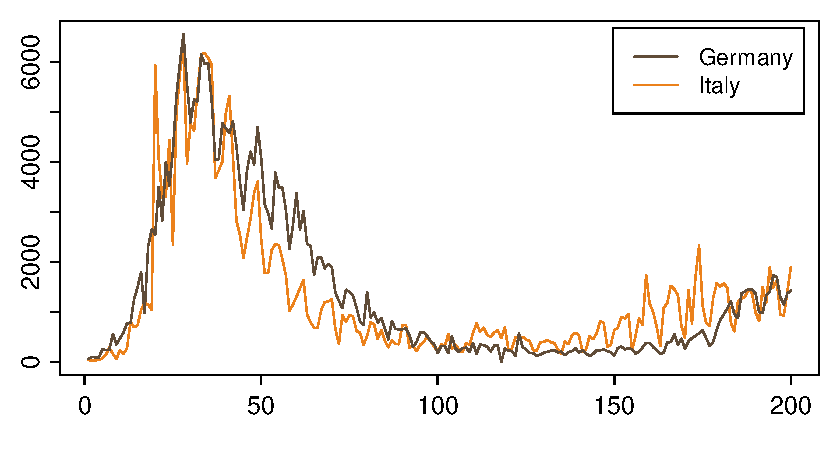
\includegraphics[height=0.45\textheight]{plots/Germany_and_Italy.pdf}
    		%\caption{Observed new cases per day in Germany and Italy}
    		\label{fig:DEUvsITA}
  	\end{figure}\pause
	\vspace{-3mm}
	\begin{block}{Aim of the paper}
	To develop new inference methods that allow to \textit{identify} and \textit{locate} differences between time trends.
	\end{block}
\end{frame}

\section{Model}
\begin{frame}{Model}
We observe $n$ time series $\mathcal{X}_i = \{X_{it}: 1 \le t \le T \}$ of length $T$:
\begin{equation*}
X_{it} = \lambda_i \Big( \frac{t}{T} \Big) + \sigma\sqrt{\lambda_i \Big( \frac{t}{T} \Big)} \eta_{it},
\end{equation*}\pause
\vspace{-3mm}
where
\begin{itemize}
\item $\lambda_i$ are unknown trend functions on $[0,1]$;
\item $\sigma$ is the overdispersion parameter;
\item $\eta_{it}$ are error terms that are independent across $i$ and $t$ and have zero mean and unit variance.
\end{itemize}
\end{frame}

\begin{frame}{Literature}
	Curve comparisons
	\begin{itemize}
		\item Park et al. (2009)
	\end{itemize}\pause
	Studies of COVID-19
	\begin{itemize}
		\item SEIR models
	\end{itemize}
\end{frame}

\section{The multiscale testing method}
\begin{frame}{Testing problem}

Let $\mathcal{F} =\{ \mathcal{I}_k \subseteq [0, 1]: 1 \le k \le K\}$ be a family of intervals on $[0, 1]$, and for a given interval $\mathcal{I}_k$ we want to test whether the functions $\lambda_i$ and $\lambda_j$ are the same on this interval. Formally, the testing problem is
\begin{align*}
H_0^{(ijk)}:\quad  \lambda_i(w) = \lambda_j(w) \text{ for all } w\in \mathcal{I}_k.
\end{align*}\pause
We want to test these hypothesis $H_0^{(ijk)}$ simultaneously for all pairs of countries $i$ and $j$ and all intervals $\mathcal{I}_k$ in the family $\mathcal{F}$.
\end{frame} 


\begin{frame}{Test statistic}
For the given interval $\mathcal{I}_k$ and a pair of time series $i$ and $j$ we calculate
\begin{equation*}
\hat{s}_{ijk,T} = \frac{1}{\sqrt{T h_k}} \sum\limits_{t=1}^T \ind (X_{it} -X_{jt}), 
\end{equation*}
%\vspace{-3mm}
where $h_k$ is the length of the interval $\mathcal{I}_k$. \pause Under certain assumptions, 
\begin{align*}
\Var(\hat{s}_{ijk,T})  & = \frac{\sigma^2}{Th_k} \sum\limits_{t=1}^T \ind \Big\{ \lambda_i\Big(\frac{t}{T}\Big) + \lambda_j\Big(\frac{t}{T}\Big) \Big\}. 
\end{align*}\pause
In order to normalize the variance of the statistic $\hat{s}_{ijk,T}$, we scale it by an estimator of its variance:
\[ \widehat{\Var(\hat{s}_{ijk,T})} = \frac{\hat{\sigma}^2}{Th_k} \sum\limits_{t=1}^T \ind (X_{it} + X_{jt} ), \]
with $\hat{\sigma}^2 = n^{-1} \sum_{i = 1}^n \hat{\sigma}_i^2$ and $\hat{\sigma}_i^2 = \frac{\sum_{t=2}^T (X_{it}-X_{it-1})^2}{2 \sum_{t=1}^T X_{it}}$.\hyperlink{frame_sigma}{\beamerbutton{Idea}}
\end{frame}


\begin{frame}[label = frame_teststatistic]{Test statistic}
Test statistic for the hypothesis $H_0^{(ijk)}$ is defined as
\begin{equation*}
\widehat{\psi}_{ijk, T} = \frac{\sum\nolimits_{t=1}^T \indsmall (X_{it} -X_{jt})}{\hat{\sigma} \big\{ \sum\nolimits_{t=1}^T \indsmall  (X_{it} + X_{jt} )\big\}^{1/2}}. 
\end{equation*} \pause
Under certain conditions and under the null, $\widehat{\psi}_{ijk, T}$ can be approximated by the Gaussian version of the test statistic:
\begin{align*}
\phi_{ijk,T}(u,h) = \frac{1}{\sqrt{2 T h_k}} \sum\limits_{t=1}^T \ind (Z_{it} - Z_{jt}), 
\end{align*}
where $Z_{it}$ are independent standard normal random variables.
\end{frame}


\begin{frame}[label = frame_test]{Test procedure}
\begin{align*}
H_0^{(ijk)}: \quad \lambda_i(w) = \lambda_j(w) \text{ for all } w \in \mathcal{I}_k.
\end{align*} \pause
\vspace{-5mm}
\begin{block}{Test procedure}
For the given significance level $\alpha \in (0,1)$ and for each $(i,j,k)$, reject $H_0^{(ijk)}$ if $|\widehat{\psi}_{ijk,T}| > c_{T,\text{Gauss}}(\alpha,h_k)$\pause, where 
\begin{itemize}
	\item $c_{T,\text{Gauss}}(\alpha,h_k) = b_k + q_{T,\text{Gauss}}(\alpha)/a_k$ is a scale-dependent critical value;\pause
	\item $a_k = \{\log(e/h_k)\}^{1/2} / \log \log(e^e / h_k)$ and $b_k = \sqrt{2 \log(1/h_k)}$ are scale-dependent constants; \hyperlink{frame_constants}{\beamerbutton{Idea}} \pause
	\item $q_{T, \text{Gauss}} (\alpha)$ is $(1-\alpha)$-quantile of the Gaussian test statistic $\Phi_T$;\pause
	\item and $ \Phi_T = \max_{(i,j,k)} a_k \big( |\phi_{ijk,T}| - b_k \big) $ the Gaussian test statistic.
\end{itemize}
\end{block}
\end{frame}

\section{Theoretical properties}
\begin{frame}{Assumptions}
\begin{itemize}
\onslide<1->\item[$\mathcal{C}1$] \label{C1} The functions $\lambda_i$ are uniformly Lipschitz continuous: $|\lambda_i(u) - \lambda_i(v)| \le L |u-v|$ for all $u, v \in [0,1]$.
\onslide<2->\item[$\mathcal{C}2$] \label{C2} $0 < \lambda_{\min} \le \lambda_i(w) \le \lambda_{\max} < \infty$ for all $w \in [0, 1]$ and all $i$. 
\onslide<3->\item[$\mathcal{C}3$] \label{C3} $\eta_{it}$ are independent both across $i$ and $t$.
\onslide<4->\item[$\mathcal{C}4$] \label{C4} $\E[\eta_{it}] = 0$, $\E[\eta_{it}^2] = 1$ and $\E[|\eta_{it}|^\theta] \le C_\theta < \infty$ for some $\theta > 4$. 
\onslide<5->\item[$\mathcal{C}5$] \label{C5} $h_{\max} = o(1/\log T)$ and $h_{\min} \ge CT^{-b}$ for some $b \in (0,1)$.
\onslide<6>\item[$\mathcal{C}6$] \label{C6} $p := \{ \# (i, j, k) \} = O(T^{(\theta/2)(1-b)-(1+\delta)})$ for some small $\delta > 0$.
\end{itemize}
\end{frame}


\begin{frame}{Theoretical properties}
\begin{prop}\label{prop-equality-1}
Denote $\mathcal{M}_0$ the set of triplets $(i, j, k)$ where $H_0^{(ijk)}$ holds true. Then under $\mathcal{C}1 - \mathcal{C}6$, it holds that 
\begin{align*}
 \Prob\Big( \forall (i,j,k) \in \mathcal{M}_0: |\hat{\psi}_{ijk,T}| \le c_{T,\textnormal{Gauss}}(\alpha,h_k) \Big) \ge 1 - \alpha + o(1)
\end{align*}
\end{prop}
\end{frame}


\begin{frame}{Strategy of the proof}
\begin{itemize}
\item Replace the statistic $\widehat{\Psi}_T$ under $H_0: m = 0$ by a statistic $\widetilde{\Phi}_T$ with the same distribution and the property that 
\begin{equation*}\label{eq-theo-stat-strategy-step1}
\big| \widetilde{\Phi}_T - \Phi_T \big| = o_p(\delta_T),
\end{equation*}
where $\delta_T = o(1)$. To do so, we make use of strong approximation theory for dependent processes as derived in Berkes et al. (2014)\pause
\vspace{2mm}
\item Using the anti-concentration results for Gaussian random vectors (Chernozhukov et al. 2015), prove that $\Phi_T$ does not concentrate too strongly in small regions of the form $[x-\delta_T,x+\delta_T]$, i.e.
\begin{equation*}\label{eq-theo-stat-strategy-step2}
\sup_{x \in \mathbb{R}} \Prob \big( |\Phi_T - x| \le \delta_T \big) = o(1).
\end{equation*}\pause
\vspace{-2mm}
\item Show that 
\begin{equation*}\label{eq-theo-stat-strategy-claim}
\sup_{x \in \mathbb{R}} \big| \Prob(\widetilde{\Phi}_T \le x) - \Prob(\Phi_T \le x) \big| = o(1). 
\end{equation*}
\end{itemize}
\end{frame}


\begin{frame}{Theoretical properties}
Define
\begin{align*}
\Pi_T^+ = \big\{ I_{u,h} = [u-h,u+h]: (u,h) \in \mathcal{A}_T^+ \text{ and } I_{u, h} \subseteq [0,1] \big\}\\
\onslide<2->{\Pi_T^- = \big\{ I_{u,h} = [u-h,u+h]: (u,h) \in \mathcal{A}_T^- \text{ and } I_{u, h} \subseteq [0,1] \big\}}
\end{align*}
\vspace{-5mm}
with
\begin{align*} 
&\mathcal{A}_T^+ = \Big\{ (u,h) \in \mathcal{G}_T: \frac{\widehat{\psi}_T(u,h)}{\widehat{\sigma}} > q_T(\alpha)  + \lambda(h)  \Big\}\\
&\onslide<2->{\mathcal{A}_T^- = \Big\{ (u,h) \in \mathcal{G}_T: -\frac{\widehat{\psi}_T(u,h)}{\widehat{\sigma}} > q_T(\alpha)  + \lambda(h)  \Big\}}
\end{align*}
\end{frame}

\begin{frame}{Theoretical properties}
\begin{prop}\label{prop-shape-3}
Under our assumptions, for events $E_T^+ = \Big\{ \forall I_{u,h} \in \Pi_T^+: m^{\prime}(v) > 0 \text{ for some } v \in I_{u,h}\Big\}$
\only<1>{ it holds that}
\onslide<2->{and $E_T^{-} = \Big\{ \forall I_{u,h} \in \Pi_T^-: m^{\prime}(v) < 0 \text{ for some } v \in I_{u,h}\Big\}$ it holds that } 
\begin{align*}
\Prob \big( E_T^+ \big) \ge (1-\alpha) + o(1)\\
\onslide<2->{\Prob \big( E_T^- \big) \ge (1-\alpha) + o(1)}
\end{align*} 
\end{prop}
\end{frame}

\begin{frame}{Graphical representation}
\begin{block}{Minimal intervals}
An interval $\mathcal{I}_k \in \mathcal{F}_{\text{reject}}(i, j)$ is called \textbf{minimal} if there is no other interval $\mathcal{I}_{k^\prime} \in \mathcal{F}_{\text{reject}}(i, j)$ with $\mathcal{I}_{k^\prime} \subset \mathcal{I}_k$. The set of minimal intervals is denoted $\mathcal{F}_{\text{reject}}^\min (i, j)$.
\end{block}\pause
Define
\begin{align*}
\Pi^{min, +}_T &= \text{ set of minimal intervals from }\Pi^+_T,\\
E_T^{min, +} &= \Big\{ \forall I_{u,h} \in \Pi_T^{min, +}: m'(v) > 0 \text{ for some } v \in I_{u,h}\Big\}
\end{align*}\pause
Since $E_T^{min, +} = E_T^{+}$, we have
\begin{align*}
\Prob \big( E_T^{min, +} \big) \ge (1-\alpha) + o(1).
\end{align*}
\end{frame}



\section{Conclusion}
\begin{frame}{Conclusion}
We developed multiscale methods to test qualitative hypotheses about nonparametric time trends:
\begin{itemize}
\item whether the trend is present at all;
\item whether the trend function is constant;
\item in which time regions there is an upward/downward movement in the trend.
\end{itemize}
We derived asymptotic theory for the proposed tests.

As an application of our method, we analyzed the behavior of the yearly mean temperature in Central England from 1659 to 2017.
\end{frame}


\begin{frame}[standout]
  Thank you!
\end{frame}




\appendix

%\begin{frame}{Simulation results of the multiscale test for constant trend function}
%\scriptsize{\begin{table}[t]
%\begin{center}
%\caption{Size of the multiscale test.}
%\label{tab:size_shape}
%% latex table generated in R 3.4.3 by xtable 1.8-2 package
% 
\begin{tabular}{cccc}
  \hline
  & \multicolumn{3}{c}{nominal size $\alpha$} \\
 $T$ & 0.01 & 0.05 & 0.1 \\
 \hline
250 & 0.004 & 0.022 & 0.082 \\ 
  350 & 0.007 & 0.031 & 0.067 \\ 
  500 & 0.011 & 0.056 & 0.086 \\ 
  1000 & 0.011 & 0.060 & 0.098 \\ 
   \hline
\end{tabular}

%\end{center}
%\end{table}}
%\begin{center}
%\normalsize{Power of the multiscale test for different slope parameters $\beta$.}
%\end{center}
%\vspace{-5mm}
%\scriptsize{\begin{columns}
%\begin{column}[b]{0.33\textwidth}
%\begin{table}[t]
%\centering
%\caption{$\beta = 1.25$}\label{tab:power_050_ll_shape}
%% latex table generated in R 3.4.3 by xtable 1.8-2 package
% 
\begin{tabular}{cccc}
  \hline
  & \multicolumn{3}{c}{nominal size $\alpha$} \\
 $T$ & 0.01 & 0.05 & 0.1 \\
 \hline
250 & 0.107 & 0.223 & 0.358 \\ 
  350 & 0.216 & 0.374 & 0.500 \\ 
  500 & 0.280 & 0.554 & 0.678 \\ 
  1000 & 0.756 & 0.910 & 0.935 \\ 
   \hline
\end{tabular}

%\end{table}
%\end{column}
%\begin{column}[b]{0.33\textwidth}
%\begin{table}[t]
%\centering
%\caption{$\beta = 1.875$}\label{tab:power_075_ll_shape}
%% latex table generated in R 3.4.3 by xtable 1.8-2 package
% 
\begin{tabular}{cccc}
  \hline
  & \multicolumn{3}{c}{nominal size $\alpha$} \\
 $T$ & 0.01 & 0.05 & 0.1 \\
 \hline
250 & 0.365 & 0.582 & 0.709 \\ 
  350 & 0.644 & 0.779 & 0.845 \\ 
  500 & 0.784 & 0.942 & 0.976 \\ 
  1000 & 0.997 & 1.000 & 1.000 \\ 
   \hline
\end{tabular}

%\end{table}
%\end{column}
%\begin{column}[b]{0.33\textwidth}
%\begin{table}[t]
%\centering
%\caption{$\beta = 2.5$}\label{tab:power_100_ll_shape}
%% latex table generated in R 3.4.3 by xtable 1.8-2 package
% 
\begin{tabular}{cccc}
  \hline
  & \multicolumn{3}{c}{nominal size $\alpha$} \\
 $T$ & 0.01 & 0.05 & 0.1 \\
 \hline
250 & 0.717 & 0.875 & 0.928 \\ 
  350 & 0.933 & 0.977 & 0.989 \\ 
  500 & 0.989 & 0.999 & 1.000 \\ 
  1000 & 1.000 & 1.000 & 1.000 \\ 
   \hline
\end{tabular}

%\end{table}
%\end{column}
%\end{columns}}
%\end{frame}

\begin{frame}
\thispagestyle{empty}
\begin{center}
\Large{\textbf{Long-run error variance estimator}}
\end{center}
\end{frame}

\begin{frame}{Setting}
Estimate the long-run error variance $\sigma^2 = \sum\nolimits_{\ell=-\infty}^{\infty} \Cov(\varepsilon_0,\varepsilon_{\ell})$ of the error terms $\{\varepsilon_t\}$ in the model 
\begin{equation*}
Y_t = m \Big( \frac{t}{T} \Big) + \varepsilon_t, 
\end{equation*}
where $\{\varepsilon_t\}$ is a stationary and causal AR($p$) process of the form 
\begin{equation*}
\varepsilon_t = \sum_{j=1}^p a_j \varepsilon_{t-j} + \eta_t. 
\end{equation*} \pause
\begin{itemize}
	\item $\boldsymbol{a} = (a_1,\ldots,a_p)$ is a vector of the unknown parameters;\pause
	\item $\eta_t$ are i.i.d.\ innovations with $\E[\eta_t] = 0$ and $\E[\eta_t^2] = \nu^2$;\pause
	\item $p$ is known.
\end{itemize}
\end{frame}

\begin{frame}{Estimator, first stage}
Yule-Walker equations yield 
\begin{equation*}\label{YU-eq}
\boldsymbol{\Gamma}_q \boldsymbol{a} = \boldsymbol{\gamma}_q + \nu^2 \boldsymbol{c}_q,  
\end{equation*} 
where
\vspace{-3mm}
\begin{itemize}
	\item $\boldsymbol{c}_q = (c_{q-1},\dots,c_{q-p})^\top$ are the coefficients from the MA($\infty$) expansion of $\{ \varepsilon_t \}$;\pause
	\item $\boldsymbol{\gamma}_q = (\gamma_q(1),\dots,\gamma_q(p))^\top$ with $\gamma_q(\ell) = \Cov(\Delta_q \varepsilon_t,$ $\Delta_q \varepsilon_{t-\ell})$;\pause
	\item and $\boldsymbol{\Gamma}_q$ is the $p \times p$ covariance matrix $\boldsymbol{\Gamma}_q = (\gamma_q(i-j): 1 \le i,j \le p)$.
\end{itemize}\pause
\begin{block}{Note}
\vspace{-3mm}
\begin{center}
$\boldsymbol{\Gamma}_q \boldsymbol{a} \approx \boldsymbol{\gamma}_q$ for large values of $q$.
\end{center}\vspace{-3mm}\end{block}\pause
\vspace{-3mm}

We construct the first-stage estimator by
\begin{equation*}
\widetilde{\boldsymbol{a}}_q = \widehat{\boldsymbol{\Gamma}}_q^{-1} \widehat{\boldsymbol{\gamma}}_q, 
\end{equation*}
where $\widehat{\boldsymbol{\Gamma}}_q$ and $\widehat{\boldsymbol{\gamma}}_q$ are constructed from the sample autocovariances $\widehat{\gamma}_q(\ell) = (T-q)^{-1} \sum_{t=q+\ell+1}^T \Delta_q Y_{t,T} \Delta_q Y_{t-\ell,T}$. 
\end{frame}

\begin{frame}{Estimator, second stage}
\begin{block}{Problem}
If the trend $m$ is pronounced, the estimator $\widetilde{\boldsymbol{a}}_q$ will have a strong bias.
\end{block}\pause
\vspace{-2mm}
Solution:
\begin{itemize}
	\item \vspace{-2mm} Compute estimators $\widetilde{c}_k$ of $c_k$ based on $\widetilde{\boldsymbol{a}}_q$.\pause
	\item Estimate the innovation variance $\nu^2$ by $\widetilde{\nu}^2 = (2T)^{-1} \sum_{t=p+1}^T \widetilde{r}_{t,T}^2$, where $\widetilde{r}_{t,T} = \Delta_1 Y_{t,T} - \sum_{j=1}^p \widetilde{a}_j \Delta_1 Y_{t-j,T}$.\pause
	\item Estimate $\boldsymbol{a}$ by 
\begin{equation*}\label{est-AR-SS} 
\widehat{\boldsymbol{a}}_r = \widehat{\boldsymbol{\Gamma}}_r^{-1} (\widehat{\boldsymbol{\gamma}}_r + \widetilde{\nu}^2 \widetilde{\boldsymbol{c}}_r).
\end{equation*}\pause
	\item \vspace{-2mm} Average the estimators $\widehat{\boldsymbol{a}}_r$: $\widehat{\boldsymbol{a}} = \frac{1}{\overline{r}} \sum\limits_{r=1}^{\overline{r}} \widehat{\boldsymbol{a}}_r$.\pause
	\item Estimate the long-run variance $\sigma^2$ by 
\begin{equation*} \label{est-lrv}
\widehat{\sigma}^2 = \frac{\widehat{\nu}^2}{(1 - \sum_{j=1}^p \widehat{a}_j)^2}. 
\end{equation*}
\end{itemize}
\end{frame}



\begin{frame}{Motivation for the estimator}
If $\{\varepsilon_t\}$ is an AR($p$) process, then the time series $\{ \Delta_q \varepsilon_t \}$ of the differences $\Delta_q \varepsilon_t = \varepsilon_t - \varepsilon_{t-q}$ is an ARMA($p,q$) process of the form 
\begin{equation*}
\Delta_q \varepsilon_t - \sum_{j=1}^p a_j \Delta_q \varepsilon_{t-j} = \eta_t - \eta_{t-q}. 
\end{equation*}\pause

Then $\Delta_q Y_{t, T} = Y_{t, T} - Y_{t-q, T}$ is approximately an ARMA($p,q$) process.
\end{frame}

\begin{frame}{Theoretical properties of the estimator}
Performance:
\begin{itemize}
\item Our estimator $\widehat{\boldsymbol{a}}$ produces accurate estimation results even when the AR polynomial $A(z) = 1 - \sum_{j=1}^p a_j z^j$ has a root close to the unit circle.\pause
\item Our pilot estimator $\widetilde{\boldsymbol{a}}_q$ tends to have a substantial bias when the trend $m$ is pronounced. Our estimator $\widehat{\boldsymbol{a}}$ reduces this bias considerably.\pause
\end{itemize}
\begin{prop}{}
Our estimators $\widetilde{\boldsymbol{a}}_q$, $\widehat{\boldsymbol{a}}$ and $\widehat{\sigma}^2$ are $\sqrt{T}$-consistent. 
\end{prop}
\end{frame}

\begin{frame}[label = frame_lambda]{Idea behind the additive correction}
\onslide<1->{Consider the uncorrected statistic
\begin{align*}
\widehat{\Psi}_{T, \text{uncorrected}} = \max_{(u,h) \in \mathcal{G}_T} \Big|\frac{\widehat{\psi}_T(u,h)}{\widehat{\sigma}}\Big|
\end{align*}
under the null hypothesis $H_0: m = 0$ and under simplifying assumptions:
\begin{itemize}
\item the errors $\varepsilon_i$ are i.i.d. normally distributed;
\item $\widehat{\sigma} = \sigma$;
\item $\mathcal{G}_T = \{(u_k, h_l) | u_k = (2k - 1)h_l \text{ for } 1\le k \le 1/2h_l, 1 \le l \le L\}$.\pause
\end{itemize}}
\onslide<2->{\begin{align*}
\widehat{\Psi}_{T, \text{uncorrected}} = \max_{1 \le l \le L} \max_{1\le k \le 1/2h_l} \Big|{\color<3>{mLightBrown}\frac{\widehat{\psi}_T(u_k,h_l)}{\sigma}}\Big|
\end{align*}}
\onslide<4->{$\Rightarrow \quad \max_k \frac{\widehat{\psi}_T(u_k,h_l)}{\sigma} ={\color<5->{mLightBrown}\sqrt{2\log(1/2h_l)}} + o_P(1) \to \infty$ as $h \to 0$ and the stochastic behavior of $\widehat{\Psi}_{T, \text{uncorrected}}$ is dominated by $\frac{\widehat{\psi}_T(u_k,h_l)}{\sigma}$ for small bandwidths $h_l$. \hyperlink{frame_teststatistic}{\beamerbutton{Go back}}}
\end{frame}

\begin{frame}[label = frame_sigma]{Idea behind $\hat{\sigma}$}
\hyperlink{frame_teststatistic}{\beamerbutton{Go back}}
\end{frame}

\begin{frame}[label = frame_constants]{Idea behind $a_k$ and $b_k$}
\hyperlink{frame_test<4>}{\beamerbutton{Go back}}
\end{frame}

\end{document}
